\subsection{Giraph}
Giraph programs all follow a similar construct. As a minimum, the \verb/compute()/ method needs to be implemented because this is where the algorithms are executed on each vertex within the graph. Listing \ref{lst:giraphstructure} shows the structure of most of the algorithms implemented using Giraph.

As explained in Section \ref{sec:res_giraph}, a Giraph program is executed as a Hadoop job. This means that in addition to the \verb/compute()/ method being complete, other classes are required to read in and write out the graphs before and after processing to the HDFS.

\lstset{language=Java,caption={Basic structure of a Giraph program},label=lst:giraphstructure,tabsize=2,breaklines=true,breakatwhitespace=true,frame=single}
\begin{lstlisting}[float]
public class Vertex<I, V, E, M> {
	public void compute(Iterator<M> msgIterator) {}
	
	public static class VertexInputFormat {}
	
	public static class VertexReader {}
	
	public static class VertexOutputFormat {}
	
	public static class VertexWriter {}
	
	public int run(String[] argArray) {}
	
	public static void main (String[] args) {}
}						
\end{lstlisting}

The following briefly describes each of these components:

\begin{itemize}

    \item {\tt compute()}

    \begin{description}
        The method which implements the algorithm.
    \end{description}
    
    \item {\tt VertexInputFormat}

    \begin{description}
        Generates splits of the input file to distribute the graph across all workers.
    \end{description}
    
    \item {\tt VertexReader}

    \begin{description}
        Controls reading in the vertices from the input splits.
    \end{description}
    
    \item {\tt VertexOutputFormat}

    \begin{description}
        Controls the output of the graph after computation
    \end{description}
    
    \item {\tt VertexWriter}

    \begin{description}
        Controls the output of the vertices for each worker after computation.
    \end{description}
    
    \item {\tt run()}

    \begin{description}
        Controls the running of the program, including handling of command-line options.
    \end{description}
    
    \item {\tt main()}

    \begin{description}
        The initial method called when the program is submitted as a Hadoop job. Calls the {\tt run()} method.
    \end{description}
    
\end{itemize}

Following on from the shortest paths example \cite{giraphexample} provided by Apache for Giraph, the decision was taken to use the same JSON\footnote{JavaScript Object Notation \url{http://www.json.org/}} style format to store the graphs as adjacency list structures in the HDFS.

\lstset{language=C,caption={JSON adjacency list representation of a graph},label=lst:json,tabsize=2,breaklines=true,breakatwhitespace=true,frame=single}
\begin{lstlisting}[float]
[1, 0, [[2, 1], [3, 1]]]
[2, 0, [[1, 1], [3, 1]]]
[3, 0, [[1, 1], [2, 1], [4, 1]]]
[4, 0, [[3, 1], [5, 1], [6, 1]]]
[5, 0, [[4, 1], [6, 1]]]
[6, 0, [[4, 1], [5, 1]]]
\end{lstlisting}

Listing \ref{lst:json} represents the graph shown in Figure \ref{fig:json}. The adjacency list representation can be split into three parts, the vertex ID, the vertex value, and a list edges this vertex connects to. As explained in Section \ref{sec:res_giraph}, Giraph only processes directed graphs, hence the need to represent edges in both directions to simulate an undirected graph. The use of this JSON format also maps quite neatly onto the structure of the \verb/Vertex/ class representing a vertex within Giraph, as the vertex ID, vertex value and edges are all easily obtainable.

\begin{figure}[htbp]
  \centering
    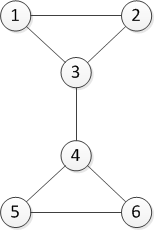
\includegraphics{./img/json}
  \caption{The graph represented by Listing \ref{lst:json}}
  \label{fig:json}
\end{figure}

Listings \ref{lst:giraphvertexinput}-\ref{lst:giraphvertexwriter} show example implementations of the classes VertexInputFormat, VertexReader, VertexOutputFormat and VertexWriter found in Listing \ref{lst:giraphstructure}. The VertexInputFormat and VertexOutputFormat classes are opposite in how they operate. The VertexInputFormat class found in Listing \ref{lst:giraphvertexinput} 


\lstset{language=Java,caption={Giraph example VertexInputFormat \cite{giraphexample} },label=lst:giraphvertexinput,tabsize=2,breaklines=true,breakatwhitespace=true,frame=single}
\begin{lstlisting}[float]
public static class SimpleShortestPathsVertexInputFormat extends
        TextVertexInputFormat<LongWritable, DoubleWritable, FloatWritable> {
    @Override
    public VertexReader<LongWritable, DoubleWritable, FloatWritable>
            createVertexReader(InputSplit split,
                               TaskAttemptContext context)
                               throws IOException {
        return new SimpleShortestPathsVertexReader(
            textInputFormat.createRecordReader(split, context));
    }
}
\end{lstlisting}

\lstset{language=Java,caption={Giraph example VertexOutputFormat \cite{giraphexample} },label=lst:giraphvertexoutput,tabsize=2,breaklines=true,breakatwhitespace=true,frame=single,showstringspaces=false}
\begin{lstlisting}[float]
public static class SimpleShortestPathsVertexOutputFormat extends
        TextVertexOutputFormat<LongWritable, DoubleWritable,
        FloatWritable> {

    @Override
    public VertexWriter<LongWritable, DoubleWritable, FloatWritable>
            createVertexWriter(TaskAttemptContext context)
            throws IOException, InterruptedException {
        RecordWriter<Text, Text> recordWriter =
            textOutputFormat.getRecordWriter(context);
        return new SimpleShortestPathsVertexWriter(recordWriter);
    }
}
\end{lstlisting}

\lstset{language=Java,caption={Giraph example VertexReader \cite{giraphexample} },label=lst:giraphvertexreader,tabsize=2,breaklines=true,breakatwhitespace=true,frame=single,showstringspaces=false}
\begin{lstlisting}[float]
public static class SimpleShortestPathsVertexReader extends
        TextVertexReader<LongWritable, DoubleWritable, FloatWritable> {

    public SimpleShortestPathsVertexReader(
            RecordReader<LongWritable, Text> lineRecordReader) {
        super(lineRecordReader);
    }
    @Override
    public boolean next(MutableVertex<LongWritable,
                        DoubleWritable, FloatWritable, ?> vertex)
            throws IOException, InterruptedException {
        if (!getRecordReader().nextKeyValue()) {
            return false;
        }
        Text line = getRecordReader().getCurrentValue();
        try {
            JSONArray jsonVertex = new JSONArray(line.toString());
            vertex.setVertexId(
                new LongWritable(jsonVertex.getLong(0)));
            vertex.setVertexValue(
                new DoubleWritable(jsonVertex.getDouble(1)));
            JSONArray jsonEdgeArray = jsonVertex.getJSONArray(2);
            for (int i = 0; i < jsonEdgeArray.length(); ++i) {
                JSONArray jsonEdge = jsonEdgeArray.getJSONArray(i);
                Edge<LongWritable, FloatWritable> edge =
                    new Edge<LongWritable, FloatWritable>(
                        new LongWritable(jsonEdge.getLong(0)),
                        new FloatWritable((float) jsonEdge.getDouble(1)));
                vertex.addEdge(edge);
            }
        } catch (JSONException e) {
            throw new IllegalArgumentException(
                ``next: Couldn't get vertex from line `` + line, e);
        }
        return true;
}}
\end{lstlisting}

\lstset{language=Java,caption={Giraph example VertexWriter \cite{giraphexample} },label=lst:giraphvertexwriter,tabsize=2,breaklines=true,breakatwhitespace=true,frame=single,showstringspaces=false}
\begin{lstlisting}[float]
public static class SimpleShortestPathsVertexWriter extends
        TextVertexWriter<LongWritable, DoubleWritable, FloatWritable> {
    public SimpleShortestPathsVertexWriter(
            RecordWriter<Text, Text> lineRecordWriter) {
        super(lineRecordWriter);
    }

    @Override
    public void writeVertex(BasicVertex<LongWritable, DoubleWritable,
                            FloatWritable, ?> vertex)
            throws IOException, InterruptedException {
        JSONArray jsonVertex = new JSONArray();
        try {
            jsonVertex.put(vertex.getVertexId().get());
            jsonVertex.put(vertex.getVertexValue().get());
            JSONArray jsonEdgeArray = new JSONArray();
            for (Edge<LongWritable, FloatWritable> edge :
                    vertex.getOutEdgeMap().values()) {
                JSONArray jsonEdge = new JSONArray();
                jsonEdge.put(edge.getDestVertexId().get());
                jsonEdge.put(edge.getEdgeValue().get());
                jsonEdgeArray.put(jsonEdge);
            }
            jsonVertex.put(jsonEdgeArray);
        } catch (JSONException e) {
            throw new IllegalArgumentException(
                "writeVertex: Couldn't write vertex " + vertex);
        }
        getRecordWriter().write(new Text(jsonVertex.toString()), null);
    }
}
\end{lstlisting}